% *======================================================================*
%  Cactus Thorn template for ThornGuide documentation
%  Author: Ian Kelley
%  Date: Sun Jun 02, 2002
%  $Header$
%
%  Thorn documentation in the latex file doc/documentation.tex
%  will be included in ThornGuides built with the Cactus make system.
%  The scripts employed by the make system automatically include
%  pages about variables, parameters and scheduling parsed from the
%  relevant thorn CCL files.
%
%  This template contains guidelines which help to assure that your
%  documentation will be correctly added to ThornGuides. More
%  information is available in the Cactus UsersGuide.
%
%  Guidelines:
%   - Do not change anything before the line
%       % START CACTUS THORNGUIDE",
%     except for filling in the title, author, date, etc. fields.
%        - Each of these fields should only be on ONE line.
%        - Author names should be separated with a \\ or a comma.
%   - You can define your own macros, but they must appear after
%     the START CACTUS THORNGUIDE line, and must not redefine standard
%     latex commands.
%   - To avoid name clashes with other thorns, 'labels', 'citations',
%     'references', and 'image' names should conform to the following
%     convention:
%       ARRANGEMENT_THORN_LABEL
%     For example, an image wave.eps in the arrangement CactusWave and
%     thorn WaveToyC should be renamed to CactusWave_WaveToyC_wave.eps
%   - Graphics should only be included using the graphicx package.
%     More specifically, with the "\includegraphics" command.  Do
%     not specify any graphic file extensions in your .tex file. This
%     will allow us to create a PDF version of the ThornGuide
%     via pdflatex.
%   - References should be included with the latex "\bibitem" command.
%   - Use \begin{abstract}...\end{abstract} instead of \abstract{...}
%   - Do not use \appendix, instead include any appendices you need as
%     standard sections.
%   - For the benefit of our Perl scripts, and for future extensions,
%     please use simple latex.
%
% *======================================================================*
%
% Example of including a graphic image:
%    \begin{figure}[ht]
% 	\begin{center}
%    	   \includegraphics[width=6cm]{MyArrangement_MyThorn_MyFigure}
% 	\end{center}
% 	\caption{Illustration of this and that}
% 	\label{MyArrangement_MyThorn_MyLabel}
%    \end{figure}
%
% Example of using a label:
%   \label{MyArrangement_MyThorn_MyLabel}
%
% Example of a citation:
%    \cite{MyArrangement_MyThorn_Author99}
%
% Example of including a reference
%   \bibitem{MyArrangement_MyThorn_Author99}
%   {J. Author, {\em The Title of the Book, Journal, or periodical}, 1 (1999),
%   1--16. {\tt http://www.nowhere.com/}}
%
% *======================================================================*

% If you are using CVS use this line to give version information
% $Header$

\documentclass{article}

\usepackage{graphicx}
\usepackage{url}
\usepackage{hyperref}

\begin{document}

% The author of the documentation
\author{Roland Haas \textless rhaas@illinois.edu\textgreater}

% The title of the document (not necessarily the name of the Thorn)
\title{POWER}

% the date your document was last changed, if your document is in CVS,
% please use:
%    \date{$ $Date: 2004-01-07 15:12:39 -0500 (Wed, 07 Jan 2004) $ $}
\date{May 13 2021}

\maketitle

% Do not delete next line
% START CACTUS THORNGUIDE

% Add all definitions used in this documentation here
%   \def\mydef etc

% Add an abstract for this thorn's documentation
\begin{abstract}
POWER is an open source, Python package to monitor the status and progress of
numerical relativity simulations, and to post-process the data products of
these simulations to compute the gravitational wave strain at future null
infinity.
\end{abstract}

% The following sections are suggestive only.
% Remove them or add your own.

\section{Introduction}
POWER takes multipolar output of the Weyl scalar $\psi_4^{\ell,m}$ extracted
on spheres of finite radius and compute the strain $h^{\ell,m}$ at
$\mathcal{I}^+$. POWER provides different interfaces to its functionality,
via either a command line interface designed to be easy to use and cover the
typical use from within the Einstein Toolkit and a Python module interface
that exposes the full capabilities of the code.

\section{Physical System}

At distances far away from sources of gravity when spacetime locally
approaches flat spacetime the gravitational wave strain is linked to the
outgoing wave Weyl scalar $\psi_4$ by~\cite{POWER-Reisswig:2010di}:

\begin{equation}
\psi_4 = \ddot h_{+} - i \ddot h_{\times}
\label{eqn:psi4fromstrain}
\end{equation}

in terms of the cross $\times$ and plus $+$ polarizations of the gravitational
wave strain $h$.

Similarly, in a neighbourhood of $\mathcal{I}^+$ one has the Peeling
theorem~\cite{POWER-Wald:1984rg,POWER-Hinder:2011xx} which states

\begin{equation}
\psi_4 \propto r^{-1} \textrm{.}
\label{eqn:peeling}
\end{equation}

At finite distance neither of these relations is strictly true.

\section{Numerical Implementation}

Multiple ways of computing strain $h$ from the Weyl scalar $\psi_4$ and to
compute quantities at $\mathcal{I}^+$ given quantities at finite radii
exists~\cite{POWER-Taylor:2013zia, POWER-Nakano:2015pta}.

\subsection{POWER method}\label{sec:power-method}

In the extrapolation method the complex multipole moments
$\psi_4^{\ell,m}(t,r)$ computed on coordinate spheres of different radii are
first integrated twice using the fixed-frequency integration method
of~\cite{POWER-Reisswig:2010di}:

\begin{equation}
h^{\ell,m} =
-\mathcal{F}^{-1}\left[
  \mathcal{F}\left[\psi_4^{\ell,m}\right] /
  \mathop{max}(\omega_0,\omega)^2
\right]
\label{eqn:ffi}
\end{equation}

in order to obtain a strain $h^{\ell,m}(t,r)$. Here $\mathcal{F}[f]$ and
$\mathcal{F}^{-1}[f]$ are the
Fourier transform of function $f(t)$ and the inverse transform respectively.

Strain is then decomposed into amplitude and phase

\begin{equation}
h^{\ell,m} = A^{\ell,m}/r e^{i \phi_{\ell,m}}
\label{eqn:ampphase}
\end{equation}

and expressed in terms of retarded time $t_{\textrm{ret}}$

\begin{equation}
t_{\textrm{ret}} = t - r_{\star}\textrm{,}
\label{eqn:tret}
\end{equation}

where

\begin{equation}
r_{\star} = r + 2 M \ln \left( \frac{r}{2 M} - 1 \right)\textrm{.}
\label{eqn:rstar}
\end{equation}

These are then separately fit to polynomial expressions of the form:

\begin{equation}
A^{\ell,m} \approx \sum_{k=0}^{k_{\phi,\textrm{max}}} A_{(k)}^{\ell,m} r^{-k}\textrm{,}
\label{eqn:Afit}
\end{equation}

and

\begin{equation}
\phi^{\ell,m} \approx \sum_{k=0}^{k_{\phi,\textrm{max}}} \phi_{(k)}^{\ell,m} r^{-k}\textrm{.}
\label{eqn:phifit}
\end{equation}

Finally the extrapolated strain at $\mathcal{I}^+$ is computed from the
$0$\textsuperscript{th} coefficients

\begin{equation}
r h^{\ell,m} = A_{(0)}^{\ell,m} e^{i \phi_{(0)}^{\ell,m}}\textrm{.}
\label{eqn:exptrapolated-strain}
\end{equation}

POWER uses $k_{A,\textrm{max}} = 2$, $k_{\phi,\textrm{max}} = 1$.

\subsection{Nakano method}

This method implements the perturbative method described
in~\cite{POWER-Nakano:2015pta} for a Kerr background spacetime.

Integrals are computed used the fixed-frequency integration
method~\cite{POWER-Reisswig:2010di} as described in
section~\ref{sec:power-method}. Derivatives are computed using the
2\textsuperscript{nd} order accurate finite difference expression provided by
Python's \texttt{numpy.gradient} function~\cite{POWER-Harris:2020xlr}.

\section{Using This Script}

The script can be used either as a command line tool \texttt{power.py} or by
loading it as a Python module \texttt{import power}.

The former provides a simple user interface suitable for mostly automated use,
while the Python interface provides access to all options and functionality at
the price of requiring more manual work.

\begin{verbatim}
curl -O GW150914_28.tar.bz2 \
  'https://zenodo.org/record/155394/files/GW150914_28.tar.bz2?download=1'
tar -vjxf GW150914_28.tar.bz2 \
    GW150914_28/output-000{0..4}/GW150914_28/mp_psi4.h5\
    GW150914_28/output-000{0..4}/GW150914_28/quasilocalmeasures-qlm_scalars..asc \
    GW150914_28/output-0000/GW150914_28/TwoPunctures.bbh \
    GW150914_28/SIMFACTORY/properties.ini
\end{verbatim}


\subsection{Command line usage}

Please consult the output of \verb|power.py --help| for details on the
supported command line options.

\begin{verbatim}
./power.py --radii '[2:5]' --method POWER GW150914_28
\end{verbatim}

\subsection{Python usage}

Please consult the output of \verb|help(power.POWER)| and
\verb|help(power.NakanoKerr)| for details on the
supported Python options.

\begin{verbatim}
import power
import numpy

radii = [136.0, 167.0, 214.0, 300.]
modes = [(2,2)]
strains = power.POWER("GW150914_28", radii, modes)

numpy.savetxt("strain.dat", strains[None][(2,2)])
\end{verbatim}

\subsection{Example output}
Figure~\ref{fig:strain22} shows typical output produced by POWER for a binary
black holes system.

\begin{figure}[htbp!]
\centering
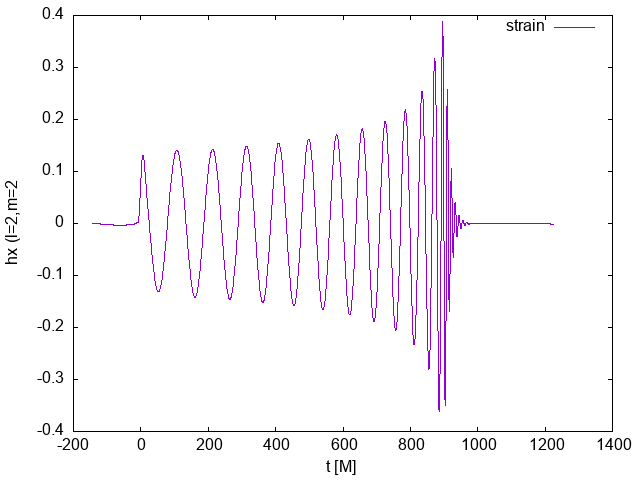
\includegraphics[width=8cm]{strain_22}
\caption{2-2 mode of strain of \texttt{GW150914\_28} gallery example.}\label{fig:strain22}
\end{figure}

\subsubsection{Computing radiated quantities}\label{sec:radiated-quantities}

POWER's output can be used to compute radiated quantities similar
to~\cite{POWER-pyGWAnalysis:web} using expressions for radiated energy and
angular momentum~\cite{POWER-Damour:2011fu}:

\begin{eqnarray}
\Delta E  &=& \frac{1}{16\pi} \int_{t_{0}}^{t} \sum_{m=-\ell}^{\ell} \sum_{\ell=2}^{\ell_{\max}} \mathrm{d}t^{\prime} \left| N_{\ell,m} \left(t^{\prime}\right) \right|^2\,,
\label{eqn:energy}\\
\Delta J  &=& \frac{1}{16\pi} \int_{t_{0}}^{t} \sum_{m=-\ell}^{\ell} \sum_{\ell=2}^{\ell_{\max}} \mathrm{d}t^{\prime} m \Im \left[h_{\ell,m}\left(t^{\prime}\right) N^{*}_{\ell,m} \left(t^{\prime}\right)\right]\,,
\label{eqn:angmom}
\end{eqnarray}

where $N_{\ell,m}$ is the news function related to the outgoing Weyl scalar by $\psi_4^{\ell,m} = \dot N_{\ell,m}$.

\paragraph{Radiated energy}

Energy radiated to infinity can be computed using Python code like this:

\begin{verbatim}
import numpy
import scipy.integrate
import glob

fn = "GW150914_N28_extrapolated_strain_l[2-9]*.dat"
paths = glob.glob("./Extrapolated_Strain/GW150914_N28/"+fn)

energy = None
for path in paths:
    strain = numpy.loadtxt(path)
    t = strain[:,0]
    h = strain[:,1] + 1.j*strain[:,2]
    dh = numpy.gradient(h, t)
    norm2 =(dh*numpy.conj(dh)).real
    
    if energy is None:
        energy = numpy.zeros_like(t)
    energy += scipy.integrate.cumulative_trapezoid(norm2, t)
energy *= 1./(16.*numpy.pi)

data = numpy.column_stack([t, energy])
numpy.savetxt("GW150914_N28_radiated_energy.dat", data)
\end{verbatim}

\subsection{Obtaining This Script}

The script is available at NCSA's Gitlab server
\url{https://git.ncsa.illinois.edu/elihu/Gravitational_Waveform_Extractor}.

\subsection{Special Behaviour}

Passing the \texttt{TwoPunctures} for the fixed-frequency integration cutoff
frequency, or ADM mass  and \texttt{QuasiLocalMeasures} for the final mass and
spin command line arguments respectively will read these quantities from
output files produced by those thorns.

A number of advanced options are accessible only as Python package variables
and required using POWER via its Python interface.

\begin{description}
\item[\texttt{OUTPUT\_DIR\_GLOB}] is a shell glob used to find all output
segment directories inside of a simulation main directory. Default:
\texttt{output-????/*} which matches SimFactory's~\cite{POWER-SimFactory:web}
layout.
\item[\texttt{PSI4\_GLOB}] the name (without extension) of the file containing
$\psi_4$ data. This can be set as the \texttt{psi4\_glob} option of \texttt{POWER},
\texttt{KerrNakano} and \texttt{getPsi4ModesInSim}. Default:
\texttt{mp\_[Pp]si4}.
\item[\texttt{JUNK\_TIME}] the time after which initial junk radiation has
left the vicinity of the coordinate origin. This time is used when adapting
the complex phase compute from real and imaginary parts to avoid jumps by
$2\pi$. Default: \texttt{50}.
\item[\texttt{FROM\_TWOPUNCTURES}] string constant used by \texttt{POWER} and
\texttt{KerrNakano} to indicate to read the cutoff frequency \texttt{f0} and /
or ADM mass \texttt{ADMMass} from output files.
\item[\texttt{FROM\_QUASILOCALMEASURES}]  string constant used by 
\texttt{KerrNakano} to indicate to read the final mass \texttt{M\_final} and /
or spin parameter \texttt{a\_final} from output files.
\end{description}

\subsection{Interaction With Einstein Toolkit Thorns}

POWER accepts data for the Weyl scalar $\psi_4$ in either ASCII or HDF5 file
format in the manner produced by the Multipole~\cite{POWER-Multipole:web}
thorn. Masses and spins needed for the computation can be either specified
explicitly or read from output files produced by
TwoPunctures~\cite{POWER-TwoPunctures:web} and
QuasiLocalMeasures~\cite{POWER-QuasiLocalMeasures:web}.

A typical parameter file fragment to produce all used output files looks like
this (taken from the GW150914 gallery
example~\cite{POWER-wardell_barry_2016_155394}:

\begin{verbatim}
ActiveThorns = "
  Multipole
  QuasiLocalMeasures
  TwoPunctures
  WeylScal4
"

################################################################
# Initial data
################################################################

ADMBase::initial_data  = "twopunctures"
ADMBase::initial_lapse = "twopunctures-averaged"

################################################################
# Psi4 computation
################################################################

WeylScal4::fdOrder          = 8
WeylScal4::calc_scalars     = "psis"
WeylScal4::calc_invariants  = "always"

################################################################
# Psi4 mode decomposition
################################################################

# Radii are chosen to be evenly spaced in 1/r as that is the
# variable extrapolation is performed in
Multipole::nradii       = 7
Multipole::radius[0]    = 100 # c
Multipole::radius[1]    = 115
Multipole::radius[2]    = 136
Multipole::radius[3]    = 167
Multipole::radius[4]    = 214
Multipole::radius[5]    = 300
Multipole::radius[6]    = 500
Multipole::ntheta       = 120
Multipole::nphi         = 240
Multipole::variables    = "
 WeylScal4::Psi4r{sw=-2 cmplx='WeylScal4::Psi4i' name='psi4'}
"
# choose a number for $wave_extract_every here
Multipole::out_every    = $wave_extract_every
Multipole::l_max        = 8
Multipole::output_hdf5  = yes

# Disable ASCII output to avoid creating a large number of
# files
Multipole::output_ascii = no

################################################################
# Isolated Horizons (used only by Nakano method)
################################################################

QuasiLocalMeasures::verbose                = no
QuasiLocalMeasures::veryverbose            = no
QuasiLocalMeasures::interpolator           =
  "Lagrange polynomial interpolation"
QuasiLocalMeasures::interpolator_options   = "order=4"
QuasiLocalMeasures::spatial_order          = 4
QuasiLocalMeasures::num_surfaces           = 3
QuasiLocalMeasures::surface_index      [0] = 2
QuasiLocalMeasures::surface_index      [1] = 3
QuasiLocalMeasures::surface_index      [2] = 4

\end{verbatim}

Other parameter files and thorns can be used as long as required values for
ADM mass (both methods), and final mass and spin of the resulting object
(\texttt{Nakano} method only) are provided using command line options or
function call arguments.

\subsection{Support and Feedback}

Please use the Einstein Toolkit issue system
\url{https://trac.einsteintoolkit.org} to report issues.

\subsection{Acknowledgement}

POWER benefited from SimulationTools~\cite{POWER-SimulationTools:web}.

\begin{thebibliography}{9}
\bibitem{POWER-Reisswig:2010di}
C.~Reisswig and D.~Pollney,
``Notes on the integration of numerical relativity waveforms,''
Class. Quant. Grav. \textbf{28}, 195015 (2011)
doi:10.1088/0264-9381/28/19/195015
[arXiv:1006.1632 [gr-qc]].

\bibitem{POWER-Wald:1984rg}
R.~M.~Wald,
``General Relativity,''
doi:10.7208/chicago/9780226870373.001.0001

\bibitem{POWER-Hinder:2011xx}
I.~Hinder, B.~Wardell and E.~Bentivegna,
``Falloff of the Weyl scalars in binary black hole spacetimes,''
Phys. Rev. D \textbf{84}, 024036 (2011)
doi:10.1103/PhysRevD.84.024036
[arXiv:1105.0781 [gr-qc]].

\bibitem{POWER-Taylor:2013zia}
N.~W.~Taylor, M.~Boyle, C.~Reisswig, M.~A.~Scheel, T.~Chu, L.~E.~Kidder and
B.~Szil\'agyi,
``Comparing Gravitational Waveform Extrapolation to Cauchy-Characteristic
Extraction in Binary Black Hole Simulations,''
Phys. Rev. D \textbf{88}, no.12, 124010 (2013)
doi:10.1103/PhysRevD.88.124010
[arXiv:1309.3605 [gr-qc]].

\bibitem{POWER-Nakano:2015pta}
H.~Nakano, J.~Healy, C.~O.~Lousto and Y.~Zlochower,
``Perturbative extraction of gravitational waveforms generated with Numerical
Relativity,''
Phys. Rev. D \textbf{91}, no.10, 104022 (2015)
doi:10.1103/PhysRevD.91.104022
[arXiv:1503.00718 [gr-qc]].

\bibitem{POWER-Harris:2020xlr}
C.~R.~Harris, K.~J.~Millman, S.~J.~van der Walt, R.~Gommers, P.~Virtanen, D.~Cournapeau, E.~Wieser, J.~Taylor, S.~Berg and N.~J.~Smith, \textit{et al.}
``Array programming with NumPy,''
Nature \textbf{585}, no.7825, 357-362 (2020)
doi:10.1038/s41586-020-2649-2
[arXiv:2006.10256 [cs.MS]].

\bibitem{POWER-SimulationTools:web}
I.~Hinder, B.~Wardell,
``SimulationTools,''
\url{https://simulationtools.org/}.

\bibitem{POWER-Multipole:web}
I.~Hinder,
``Multipole'',
\url{http://einsteintoolkit.org/thornguide/EinsteinAnalysis/Multipole/documentation.html}

\bibitem{POWER-QuasiLocalMeasures:web}
E.~Schnetter,
``QuasiLocalMeasures'',
\url{http://einsteintoolkit.org/thornguide/EinsteinAnalysis/QuasiLocalMeasures/documentation.html}

\bibitem{POWER-TwoPunctures:web}
M.~Ansorg, E.~Schnetter,
``TwoPunctures'',
\url{http://einsteintoolkit.org/thornguide/EinsteinInitialData/TwoPunctures/documentation.html}

\bibitem{POWER-pyGWAnalysis:web}
C.~Reisswig,
``pyGWAnalysis'',
\url{https://bitbucket.org/einsteintoolkit/pygwanalysis}

\bibitem{POWER-SimFactory:web}
``SimFactory: Herding numerical Simulations'',
\url{http://simfactory.org/}

\bibitem{POWER-Damour:2011fu}
T.~Damour, A.~Nagar, D.~Pollney and C.~Reisswig,
``Energy versus Angular Momentum in Black Hole Binaries,''
Phys. Rev. Lett. \textbf{108}, 131101 (2012)
doi:10.1103/PhysRevLett.108.131101
[arXiv:1110.2938 [gr-qc]].

\bibitem{POWER-wardell_barry_2016_155394}
B.~Wardell, I.~Hinder and E.~Bentivegna,
``Simulation of GW150914 binary black hole merger using the Einstein Toolkit,''
doi:10.5281/zenodo.155394
\url{https://doi.org/10.5281/zenodo.155394}


\end{thebibliography}

% Do not delete next line
% END CACTUS THORNGUIDE

\end{document}
